\section{Calibrating the Parameters of the Mincer Equation}


To solve the model some reasonable values for the parameters of the wage process is necessary. The wage process contains the following parameters: $(\eta_G, \eta_{G^2}, \delta, \alpha, \sigma_{\epsilon})$. As mentioned in the model specification in section \ref{sec:model1} the wage process follows the Mincer earnings equation, not accounting for education, and where the idiosyncratic wage path is added linearly to the wage. I assume that the parameters driving the wage process are the same for both men and women, and these can be by calibrated independent of the entire model. This is due to computational constraint. \textcite{friedman_elements_2001} argues that calibrating multiple parameters at the same time suffers from the \textit{curse of dimensionality}. Another more important reason is that the wage of the husband in the model is assumed perfectly deterministic, which imply I am not able to calibrate the parameters driving the wage path under the assumption these are the same for men and women. As mentioned in the model specification, the idiosyncratic wage path is added linearly. This  allows for a two-step calibration of the parameters. First calibrate $(\eta_G, \eta_{G^2}, \delta, \alpha)$ that drives the age and sex specific expected wage rate (referred to as \textit{wage path}). Second the scale of the random walk can be calibrated by $\sigma_\epsilon$ (referred to as \textit{wage variance}). In other words the parameter calibration of the income process is broken into two phases: First calibrating age and sex specific expected wage rate, second calibrating the variance of the wages. It is important to note that this is agent based modelling, where the agent is supplied with a predetermined course of action dependent on the state! 

I calibrate the wage path by using a \textbf{LONS50}, a data set from Statistics Denmark (Danmarks Statistik Bank). This data set contains the wage trend for men and women at any given age. My objective is to minimize the squared distance between the empirical wage path and the simulated wage path. The simulated wage path is constructed by simulating from the partial model with given parameters and taking the average. Certain things should be noted about this partial model. The wage path is a function of human capital which again is a function of the choice variable $H$ of the model specified in section \ref{sec:model1}. This obviously makes it problematic to calibrate the parameters. I work around the problem by using the data set \textbf{LIGEF15} containing the number of worked hours for both men and women, which is supplied by Statistics Denmark. These numbers do not take into account people leaving the labour force temporarily, which women are known to do when giving birth. I make the assumption that women leave the work force for 1 year when giving birth to a child. I use the data set \textbf{FOD33} to get fertility rates of women. Again this data is supplied by Statistics Denmark. Formally this can summed up in the policy described below:

\begin{equation}
    H_t = \begin{cases}
        H^{men}(Q) & \text{if sex=\textit{male}} \\
        H^{women}(Q) & \text{if sex=\textit{female} and birth=\textit{false}} \\
        0 & \text{if sex=\textit{female} and birth=\textit{true} }\\
    \end{cases}    
\end{equation}

The rest of the wage process follows the model described in section \ref{sec:model1}. The minimization problem follows the following process:

\begin{equation}
    \text{Cohort Average: } {\tilde{\mu}}_i (C_i) = \frac{1}{\mid C_i \mid} \sum_{\tilde{w}_{n, q} \in C_i} {\tilde{w}_{n, q}}
\end{equation}

\begin{equation}
 (\hat{\eta_G}, \hat{\eta_{G^2}}, \hat{\delta}, \hat{\alpha})   =  \underset{\eta_G, \eta_{G^2}, \delta, \alpha}{\argmin}  \frac{1}{2}\frac{1}{\mid C \mid } \sum_{C_i \in C} \lp\lp \mu_{i}^{men}(C_i)  - \tilde{\mu}_i^{men}(C_i)\rp^2 + \lp \mu_{i}^{women}(C_i)  - \tilde{\mu}_i^{women}(C_i)\rp^2 \rp
\end{equation}

Where $\tilde{w}_{n, q}$ denotes a simulated wage rate at age $q$ for the $n$'th simulated individual and $w_q$ is the true value wage rate for a given age. $C_i \in C$ denotes a given age cohort, where the age cohorts are $C=\{(20, 24), (25, 29), \cdots , (55, 59) \}$. $\mu_i$ denotes the empirical average for a given cohort.
I solve the minimization problem using Nelder-Mead (Simplex method). Essentially The simplex method allows for numerical optimization without the need to supply neither the gradient, Hessian or Jacobian matrix. I initialize the algorithm with the values: $(\alpha=4, \eta_G = 0.5, \eta_{G^2}=0.01, \delta=0.5)$, and let the algorithm run for a maximum of 100 iterations. 

Given the now calibrated parameters driving the wage path, only a single parameter $\sigma_\epsilon$ needs to be calibrated. This is again done by numerical optimization. By minimizing the mean squared error between the empirical quartiles (upper and lower) for men and women, to those found by simulating, the optimal scale for the random walk, $\sigma_\epsilon$, is found:

\begin{equation}
    \text{Cohort Quartile: } {\tilde{\omega}}_{i, j} (C_i) = \text{quartile}_j (C_i), \qquad j\in{\text{upper}, \text{lower}} 
\end{equation}

\begin{equation}\label{eq:wage_var_optimization}
   \hat{\sigma_\epsilon}  = \underset{\sigma_\epsilon}{\argmin} \frac{1}{2}\frac{1}{2}\frac{1}{\mid C \mid } \sum_{j} \sum_{sex}\sum_{C_i} \lp \omega_{i, j}^{sex}(C_i)  - \tilde{\omega}_{i,j}^{sex}(C_i)\rp^2, \qquad 
\end{equation}

Where equation \eqref{eq:wage_var_optimization} assumes $C_i \in C$, $j \in \{\text{upper},  \text{lower} \}$, and $sex \in \{\text{men}, \text{women} \}$. Again I use Nelder-Mead for optimization, set a max number of iterations of 100, and set the starting value of $\sigma_\epsilon = 0.5$. The results of the optimized parameters are listed in table \ref{tab:wage_path_optimized_params}:

\begin{table}[ht]
    \centering
    \begin{tabular}{lrrrrr}
\toprule
{} &  $\hat{\alpha}$ &  $\hat{\eta_G}$ &  $\hat{\eta_{G^{2}}}$ &  $\hat{\delta}$ &  $\hat{\sigma_{\epsilon}}$ \\
\midrule
Parameters &           4.609 &           0.164 &                 0.015 &           0.209 &                      15.11 \\
\bottomrule
\end{tabular}

    \caption{Optimized parameters for wage process}
    \label{tab:wage_path_optimized_params}
\end{table}

The parameters seem to have reasonable values comparing to other values found in the literature. First $\hat{\alpha} $ is the constant in the wage equation.
The Mincer equation is log transformed implying an $\exp (\cdot)$ transformation is required for evaluating the value. 
Assuming no human capital, $G=0$, yields $\exp (\hat{\alpha}) = \exp ( 4.609 ) \approx 100$. 
Or in other words, in this model, a totally inexperienced worker would receive an hourly wage of 100 DKK (not far from the actual minimum wage). 
Looking to $\delta$ the rate of human capital depreciation/skill atrophy, I find a value of approximately $20 \%$ per year. Compared to other studies this does seem a bit on the high side, however not unreasonable. \textcite{kunze_timing_2002} finds that parental leave reduces wages for women with about $13$ to $18 \%$ per year, while other work interruptions is about $2$  to $5 \%$ a year. \textcite{light_early-career_1995} finds values for human capital depreciation at about $13 \%$ a year. Considering the other parameters, they are harder to compare to other literature due to denomination in DKK. 


\begin{figure}[ht]

% NOTE THAT I HAVE INTERCHAGNED THE NAME OF MEN AND WOMEN
\begin{subfigure}{.5\textwidth}
  \centering
  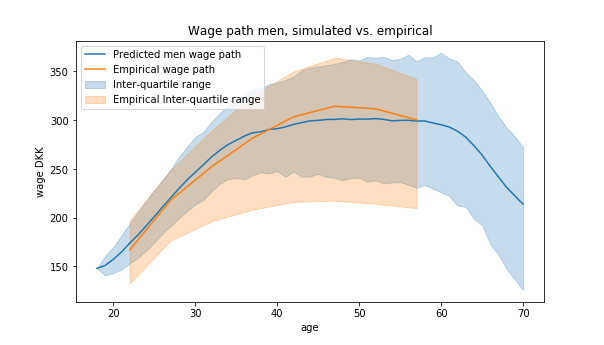
\includegraphics[width=1\linewidth]{figures/simulated_wage_path_variance_optimized_parameters_women.png}
  \caption{Men}
  \label{fig:sub1}
\end{subfigure}%
\begin{subfigure}{.5\textwidth}
  \centering
  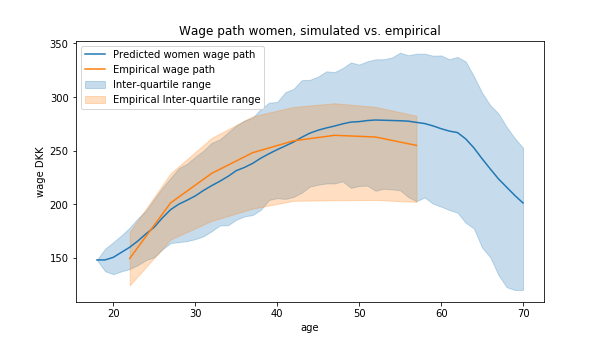
\includegraphics[width=1\linewidth]{figures/simulated_wage_path_variance_optimized_parameters_men.png}
  \caption{Women}
  \label{fig:sub2_wage_path}
\end{subfigure}
    \caption{Simulated wage process vs Empirical wage process}
    \label{fig:sim_wage_vs_empirical_wage}
\end{figure}\label{sec:parameter_calibration}

Figure \ref{fig:sim_wage_vs_empirical_wage} compares the empirical wage process with the simulated. First looking to the \textit{wage path}, I conclude that the Mincer equation seems to give a relatively good fit to the data even without taking education into account. The mean absolute error of the women wage path of women is $10.61$ DKK, and for men the number is $5.84$ DKK, which considering the relatively simple parametric form of the process, is very good. Figure \ref{fig:sim_wage_vs_empirical_wage} also  show the empirical wage process is skewed. In this formulation of the mincer equation this is not possible. The width of the inter-quartile range seem to fit the wage path of men reasonably, but for women it slightly overshoots. I conclude the parameter values of the Mincer equation do seem to yield reasonable results, and they will be used throughout the paper. A side note about the empirical wage path of men and women is that men do seem to experience a greater variance in their wage rates than women. Considering the work of both \textcite{francesconi_joint_2002} and \textcite{gayle_life-cyle_2006} that suggests that women on high income trajectories finds it less desirable to work, this is a puzzling result. The literature suggests that children could be one of the main drivers of heterogeneity observed in the wage rates of women, so when men have even higher wage rate differences, and these are not driven by children, one must conclude that other, probably equally important factors drive wage rate heterogeneity.

